\section{Solution}

In section, we describe our solution for providing privacy for prosumers without compromising the safety and security of the microgrid.
Figure~\ref{fig:softwareArchitecture} shows a high-level overview of the architecture of our solution.

\begin{figure}[h!]
\center
\begin{tikzpicture}[x=8cm, y=1.2cm,
  nodeStyle/.style={rounded corners=0.1cm, drop shadow={shadow xshift=0.05cm, shadow yshift=-0.05cm, fill=black}}
]
\draw [nodeStyle, fill=white]   (0, 0) rectangle    (1, 0.9) node [midway, align=center] {Communication network\\and operating system};

\draw [nodeStyle, fill=red!10]  (0, 1) rectangle    (1, 1.9) node [midway, align=center] {Communication anonymity\\(onion routing)};

\draw [nodeStyle, fill=blue!10] (0, 2) rectangle    (1, 2.9) node [midway, align=center] {Distributed ledger\\(blockchain)};

\draw [nodeStyle, fill=red!10]  (0,    3) rectangle (0.45, 3.9) node [midway, align=center] {Transaction anonymity\\(mixing service)};
\draw [nodeStyle, fill=blue!10] (0.47, 3) rectangle (0.72, 3.9) node [midway, align=center] {Bid storage};
\draw [nodeStyle, fill=red!10 ] (0.74, 3) rectangle (1,    3.9) node [midway, align=center] {Active\\smart meter};

\draw [nodeStyle, fill=blue!10] (0,    4) rectangle (0.49, 4.9) node [midway, align=center] {Prosumer trading\\algorithm};
\draw [nodeStyle, fill=blue!10] (0.51, 4) rectangle (1,    4.9) node [midway, align=center] {DSO control\\algorithm};
\end{tikzpicture}
\caption{High-level architecture of the proposed solution. Components marked red are introduced to provide privacy in a safe and secure manner. Components marked in blue are typical elements of a decentralized transactive microgrid.}
\label{fig:softwareArchitecture}
\end{figure}

\begin{figure*}[h]
\center
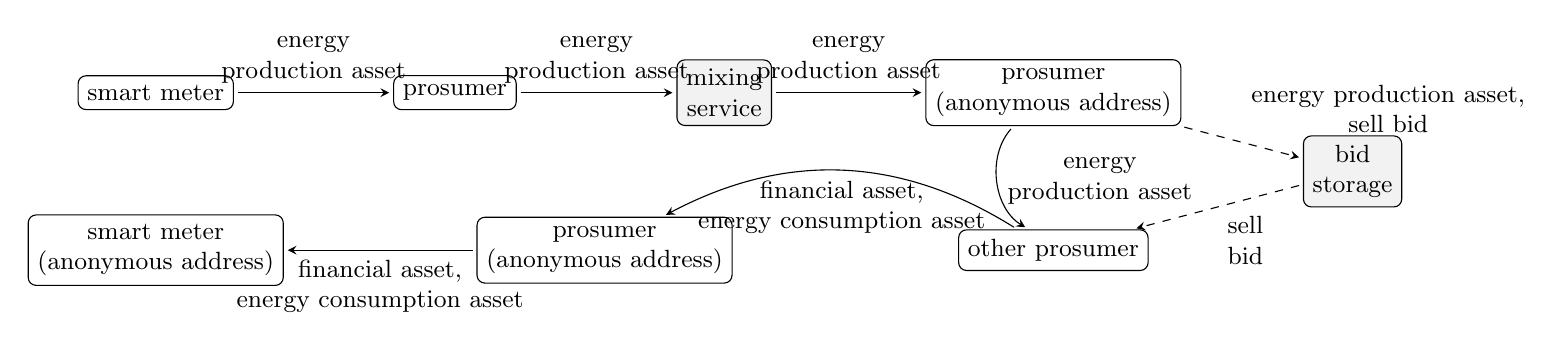
\begin{tikzpicture}[x=3.8cm, y=2cm, font=\small,
  system/.style={draw, align=center, rounded corners=0.1cm, fill=black!5},
  entity/.style={draw, align=center, rounded corners=0.1cm},
  asset/.style={midway, align=center},
  transfer/.style={->, >=stealth, shorten <=0.05cm, shorten >=0.05cm},
]
%\node[entity] (smartmeter) at (0.75, 0.5) {smart\\meter};
%\node[entity] (prosumer1) at (1.25, 1) {prosumer};
%\node[system] (mixing1) at (2, 1) {mixing\\service};
%\node[entity] (prosumer2) at (3, 1) {prosumer\\(alternative address)};
%\node[system] (bidstorage) at (4, 1) {bid\\storage};
%\node[entity] (partner) at (4, 0) {other prosumer};
%\node[entity] (prosumer3) at (3, 0) {prosumer\\(alternative address)};
%\node[system] (mixing2) at (2, 0) {mixing\\service};
%\node[entity] (prosumer4) at (1.25, 0) {prosumer};
\node[entity] (smartmeter) at (0, 1) {smart meter};
\node[entity] (prosumer1) at (1, 1) {prosumer};
\node[system] (mixing1) at (1.9, 1) {mixing\\service};
\node[entity] (prosumer2) at (3, 1) {prosumer\\(anonymous address)};
\node[system] (bidstorage) at (4, 0.5) {bid\\storage};
\node[entity] (partner) at (3, 0) {other prosumer};
\node[entity] (prosumer3) at (1.5, 0) {prosumer\\(anonymous address)};
\node[entity] (smartmeter2) at (0, 0) {smart meter\\(anonymous address)};

%\draw[transfer] (smartmeter) -- node [asset, above left] {energy\\production asset} (prosumer1);
%\draw[transfer] (prosumer1) -- node [asset, above] {energy\\production asset} (mixing1);
%\draw[transfer] (mixing1) -- node [asset, above] {energy\\production asset} (prosumer2);
%\draw[transfer, dashed] (prosumer2) -- node [asset, above] {energy production asset,\\sell bid} (bidstorage);
%\draw[transfer, dashed] (bidstorage) -- node [asset, right] {sell\\bid} (partner);
%\draw[transfer, bend right=15] (partner) to node [asset, below] {financial asset,\\energy\\consumption asset} (prosumer3);
%\draw[transfer, bend right=7.5] (prosumer2) to node [asset, above right] {energy\\prod. asset} (partner);
%\draw[transfer] (prosumer3) -- node [asset, below] {financial asset,\\
%energy consumption asset} (mixing2);
%\draw[transfer] (mixing2) -- node [asset, below] {financial asset,\\energy consumption asset} (prosumer4);
%\draw[transfer] (prosumer4) -- node [asset, below left] {financial\\asset} (smartmeter);

\draw[transfer] (smartmeter) -- node [asset, above] {energy\\production asset} (prosumer1);
\draw[transfer] (prosumer1) -- node [asset, above] {energy\\production asset} (mixing1);
\draw[transfer] (mixing1) -- node [asset, above] {energy\\production asset} (prosumer2);
\draw[transfer, dashed] (prosumer2) -- node [asset, above right] {energy production asset,\\sell bid} (bidstorage);
\draw[transfer, dashed] (bidstorage) -- node [asset, below right] {sell\\bid} (partner);
\draw[transfer, bend right=30] (partner) to node [asset, below] {financial asset,\\energy consumption asset} (prosumer3);
\draw[transfer, bend right=50] (prosumer2) to node [asset, right] {energy\\production asset} (partner);
\draw[transfer] (prosumer3) -- node [asset, below] {financial asset,\\
energy consumption asset} (smartmeter2);
\end{tikzpicture}
\caption{Simplified overview of the flow of assets from the perspective of a prosumer who sells energy production. Note that in order to prevent de-anonymization, a prosumer should use multiple addresses for mixing and multiple rounds of mixing.}
\end{figure*}

\subsection{Timing}
The ability to specify points or intervals in time is crucial.
For example, control signals specify how the load should change at certain points in time, energy trades specify when energy will be consumed or produced, etc.
To facilitate processing signals and transactions, we divide time into fixed-length intervals, and specify points or periods in time using these discrete timesteps.
The length of the time interval is determined by mapping the timing assumptions of the power system to our platform.
%In our implementation, 
For example, the default length of the time interval may be 4 seconds, which corresponds to how frequently the control signal of the DSO typically changes.

\subsection{Services}

Here, we describe three services that must be implemented for our solution: communication anonymity, mixing service for transaction anonymity, and anonymous bid storage for bidding anonymity.

\subsubsection{Communication Anonymity}
Firstly, we must provide an anonymous communication layer, on which we can build an anonymous trading platform.
Without this communication layer, bids and transactions could be easily de-anonymized based on the network identifiers of the sources (e.g., IP or MAC addresses).

We can employ well-known and widely used techniques for anonymous communication, such as \emph{onion routing}.
To build an onion network, the smart meters, inverters, and other devices can act as onion routers, and the list of onion routers in a microgrid can be published on a private blockchain.
In our first implementation, we can use the free and open-source Tor software with private Directory Authorities.
% ritter.vg: "run your own tor network"
% https://ritter.vg/blog-run_your_own_tor_network.html

\subsubsection{Transaction Anonymity}
We must provide prosumers with the ability to create and publish transactions anonymously.
More specifically, prosumers should be able to purchase or sell energy without revealing their identity; however, these transaction must also be verifiable and enforceable.

We may achieve this goal using multiple approaches for blockchain transaction anonymity:
\begin{itemize}
\item Mixing services (also known as tumblers) mix potentially identifiable assets on a blockchain with others, thereby preventing tracing individual assets back to their original source. 
In our case, assets to be mixed include virtual balances of fiat currencies as well as energy production and consumption.
\item Cryptographic anonymity for transactions is provided, for example, by Zerocoin~\cite{miers2013zerocoin}. Similarly to mixing service, Zerocoin can prevent tracing assets on a blockchain.
\end{itemize}
Using the above techniques, we can enable prosumers to trade energy anonymously (i.e., without revealing their true identities), but at the same time prevent them from altering their energy or financial balances without a valid transaction.

However, we must also ensure that 1) smart meters know the amount of energy purchased or sold by their prosumer and 2) prosumers cannot purchase or sell more energy than their capacity.
To satisfy both of these constraints, all energy trades must start with the prosumer withdrawing a certain amount of energy production or consumption from its smart meter:
\begin{itemize}
\item If a prosumer wishes to sell energy, it must first obtain an energy asset from its smart meter using a blockchain transaction.
This transaction must be signed by the smart meter, which enables the smart meter to 1) keep track of the amount of energy traded by the prosumer as well as to 2) enforce safety requirements by limiting the amount of energy that can be withdrawn.
\item If a prosumer wishes to buy energy, it must first obtain an energy consumption asset from its smart meter in a way similar to obtaining an energy production asset.
\end{itemize}

\subsubsection{Bidding Anonymity}
Finally, we must provide prosumers with the ability to publish energy buy and sell bids anonymously.
To this end, we create a storage for anonymous bids that is readable by all the prosumers in the microgrid.
Any prosumer may submit a bid to this storage; however, in order to do so, they must provide a zero-knowledge proof of owning the assets that are to be traded:
\begin{itemize}
\item To submit an energy sell bid, the prosumer must prove that it owns an energy production asset on the chain.
\item To submit an energy buy bid, the prosumer must prove that it own an energy consumption asset as well as financial assets on the chain.
\end{itemize}


\subsection{Transaction Types}

Before we can discuss transaction types, we must first define the three assets that these transactions may transfer.

An \emph{energy production asset} (EPA) is defined by
\begin{compactitem}
\item \field{power}: non-negative amount of power to produced (for example, measured in watts).
\item \field{start}: first time interval in which energy is to be produced. 
\item \field{end}: last time interval in which energy is to be produced.
\end{compactitem}
An \emph{energy consumption asset} (ECA) is defined by the same fields; however, for this asset, the fields define consumption instead of production.
Finally, a \emph{financial asset} (FA) is defined by a single non-negative field \field{amount}, which can be denominated in either a fiat currency (e.g., US dollars) or a cryptocurrency.

\subsubsection{Energy and Financial Transactions}

Energy and financial transactions transfer energy and financial asset from one address to another.
Prosumers use these transactions for multiple purposes: to trade energy by exchanging assets with other prosumers, to prove to the bid storage that they have production or consumption capacity, to hide their identity by transferring assets to and from mixing services, and to deposit assets at their smart meter.
%
An energy and financial transaction contains the following fields:
\begin{compactitem}
\item List of EPA inputs, each of which is defined by:
\begin{compactitem}
\item \field{out}: EPA output from a previous transaction,
\item \field{sig}: signature for this output.
\end{compactitem}
\item List of ECA inputs, each of which is defined by:
\begin{compactitem}
\item \field{out}: ECA output from a previous transaction,
\item \field{sig}: signature for this output.
\end{compactitem}
\item List of FA inputs, each of which is defined by:
\begin{compactitem}
\item \field{out}: FA output from a previous transaction,
\item \field{sig}: signature for this output.
\end{compactitem}
\item List of EPA outputs, each of which is defined by:
\begin{compactitem}
\item an EPA and an address to which it is transferred.
\end{compactitem}
\item List of ECA outputs, each of which is defined by:
\begin{compactitem}
\item an ECA and an address to which it is transferred.
\end{compactitem}
\item List of FA outputs, each of which is defined by:
\begin{compactitem}
\item an FA and an address to which it is transferred.
\end{compactitem}
\end{compactitem}

An energy and financial transaction is valid if the following three conditions hold.
\begin{compactitem}
\item None of the outputs referenced by the inputs have been spent by a transaction that has been recorded on the ledger.
\item All of the signatures are valid.
\item For each asset type (and for each timestep), the sum of inputs and outputs is the same.
For example, in the case of energy production assets, the condition is:
\begin{align}
\forall t: & \sum_{out \in \text{EPA outputs}} out.\mathtt{power} \cdot 1_{\left\{out.\mathtt{start} \leq t \leq out.\mathtt{end}\right\}} \nonumber \\
& = \sum_{in \in \text{EPA inputs}} in.\mathtt{out}.\mathtt{power} \cdot 1_{\left\{in.\mathtt{out}.\mathtt{start} \leq t \leq in.\mathtt{out}.\mathtt{end}\right\}} ,
\end{align}
where $1_x$ is equal to $1$ if $x$ is true, and it is $0$ otherwise.
%\begin{equation}
%\forall t: \sum_{out \in \left\{out' \middle| out' \in \text{ EPA outputs} \wedge out'.EPA.start \leq t \leq out'.EPA.end\right\}} out.EPA.Power = \sum_{in \in \left\{in' \middle| in' \in \text{ EPA inputs} \wedge in'.EPA.start \leq t \leq in'.EPA.end\right\}} in.EPA.Power .
%\end{equation}
\end{compactitem}
If a transaction submitted to the ledger is valid, it will be permanently recorded.

\subsubsection{Smart-Meter Transactions}

Prosumers use smart-meter transactions to withdraw energy and financial assets from their own smart meters, before they engage in energy trading.
%
A smart-meter transaction contains the following fields:
\begin{compactitem}
\item List of EPA outputs, each of which is defined by:
\begin{compactitem}
\item an EPA and an address to which it is transferred.
\end{compactitem}
\item List of ECA outputs, each of which is defined by:
\begin{compactitem}
\item an ECA and an address to which it is transferred.
\end{compactitem}
\item List of FA outputs, each of which is defined by:
\begin{compactitem}
\item an FA and an address to which it is transferred.
\end{compactitem}
\item \field{id}: Identifier of the smart meter.
\item \field{sig}: Smart meter's signature over the transaction.
\end{compactitem}

A smart-meter transaction is valid if the following two conditions hold:
\begin{compactitem}
\item The smart meter identified in the transaction has been authorized by a regulatory transaction that has been recorded on the ledger.
\item The smart meter's signature is valid.
\end{compactitem}
\todo{To address malfunctioning or compromised smart meters, we could also impose a limit on withdrawals.}

\subsubsection{Regulatory Transactions}

The DSO uses regulatory transactions to authorize or ban smart meters and to control the microgrid load through setting a price policy.
Since these transactions provide a diverse set of functionality, they are divided into two types.

\paragraph{Authorize or Ban Smart Meters}
The DSO uses these transactions to manage the set of authorized smart meters in the microgrid.
Whenever a new smart meter is installed, the DSO notifies the members of the microgrid using a regulatory transaction.
Similarly, whenever a smart meter is deactivated (e.g., because service is stopped or it is believed to be malfunctioning or compromised), the DSO notifies the members of the microgrid using a regulatory transaction.
These transactions contain the following fields:
\begin{compactitem}
\item List of smart meters to be authorized, each of which is defined by:
\begin{compactitem}
\item \field{id}: Identifier of the smart meter.
\item \field{pubkey}: Public key of the smart meter.
\end{compactitem}
\item List of smart meters to be banned, each of which is given using its identifier.
\item \field{time}: Timestep in which smart meters are authorized and banned.
\item \field{sig}: DSO's signature over the transaction.
\end{compactitem}

A regulatory transaction of this type is valid if the following two conditions hold:
\begin{compactitem}
\item The timestep specified in the transaction is in the future.
\item The DSO's signature is valid.
\end{compactitem}

\paragraph{Price Policy}
